\chapter{\textbf{Applications}}
    \section{Introduction}
    Nous entrons dans le dernier chapitre de ce rapport. Nous l’avons dédié aux différentes applications dans lesquelles nous avons intégré notre système de reconnaissance de plaques d’immatriculation marocaines. S’il est vrai qu’il existe plusieurs cas d’utilisation des systèmes ANPR, nous nous sommes focalisés sur deux. Le premier est une application mobile qui utilise notre système SIRAM pour lire les plaques marocaines sur les images ou des vidéos en temps réel. Le second est un parking intelligent dans lequel le système SIRAM servira à lire les plaques d’immatriculation pour donner accès ou non aux places de stationnement du parking.

    \section{Développement de l'application mobile}
Notre mission est de réaliser une simple application sous Android qui utilise le système SIRAM pour reconnaître les matricules des véhicules au Maroc sur des images ou des vidéos en temps réel. Pour réaliser une application de qualité, il est important de passer par deux étapes primordiales: l'analyse des besoins et la conception.  
    \subsection{Analyse et spécifications des besoins}
    Dans cette partie, nous allons tout simplement identifier les acteurs et leurs actions. Un acteur est une personne, une machine ou un autre système qui interagit avec le système étudié. Leurs différentes interactions avec le système constituent ce qu'on appelle cas d'utilisation.

    Pour ce qui concerne notre application, nous avons un unique acteur qui est l’\textbf{utilisateur}. Il peut accèder à l'application pour:
    \begin{itemize}
        \item \textbf{Capturer une image}: l’utilisateur peut lancer la caméra et prendre une capture d’une photo. Cette photo est ensuite automatiquement traitée par le système pour faire la reconnaissance des plaques d’immatriculation éventuellement détectées sur la photo. Le système renvoie sur l’écran de l’application le résultat en image.
        \item \textbf{Lancer le traitement en temps réel}: l’utilisateur peut encore lancer la caméra. Mais cette fois-ci, le système traite en temps réel les images reçues par la caméra. Il trace sur ces images les rectangles autour des plaques éventuelles sans oublier les numéros de matricule sur ces rectangles.
    \end{itemize}
    Pour représenter graphiquement ces fonctionnalités, nous allons utiliser ce qu’on appelle en langage UML le diagramme de cas d’utilisation. C’est un simple diagramme qui permet de décrire l’ensemble des opérations réalisables par un acteur. Ainsi notre diagramme de cas d’utilisation peut être représenté comme suit:
    \begin{figure}[H]
        \centering
        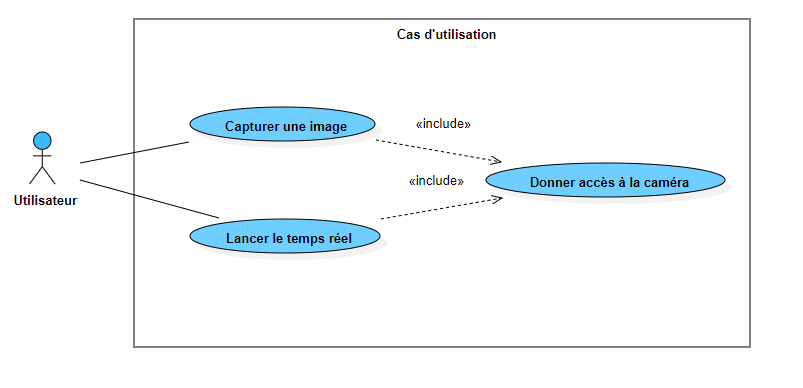
\includegraphics[scale=0.6]{useCase.png}
        \caption{Diagramme de cas d'utilisation}
    \end{figure}
    Ces fonctionnalités citées représentent les besoins fonctionnelles de notre application. Hors mis ce type de besoins, nous avons aussi les besoins non-fonctionnelles qui sont un ensemble des contraintes à respecter par l'application. Dans notre cas, on a:
    \begin{itemize}
        \item \textbf{L'ergonomie des interfaces}: les interfaces de l'application doivent être simples et conviviales pour l'utilisateur. On doit aussi limiter au maximum les encombrements.
        \item \textbf{La performance}: il s'agit principalement de la précision et la rapidité de la reconnaissance des plaques. En effet, notre application doit détecter le plus rapidement possible les plaques et identifier le numéro de plaque avec une grande précision. 
    \end{itemize}

    \subsection{Conception}
    À partir d’une bonne analyse des besoins, on réalise la conception qui est l’une sinon la plus importante étape entrant dans le processus de développement d’une application. La conception se matérialise généralement par des diagrammes UML tels que les \textbf{diagrammes de classes}, les \textbf{diagrammes de séquence} et les \textbf{diagrammes d'activités}. Un diagramme de classes permet représenter les classes et les interfaces d'un systèmes ainsi que les relations entre elles. Contrairement à un diagramme de classes qui est statique, un diagramme de séquence est dynamique et traduit les intéractions entre acteurs et/ou le système pour un cas d'utilisation déterminé. Le déroulement d'un cas d'utilisation ou d'une méthode est présentée en utilisant un diagramme d'activités.
    
    
    Pour mieux structurer notre application et faciliter ainsi les modifications et les maintenances, nous avons adopté pour une \textbf{architecture 3-tiers} (Figure \ref{fig:dc1}) c’est-à-dire composée de trois couches principales qui communiquent entre elles en offrant les services les unes aux autres:
    \begin{itemize}
        \item La \textbf{couche métier}: elle implémente la logique fonctionnelle de notre application. Elle est composée de plusieurs packages à savoir:
            \begin{itemize}
                \item[•] Le package \textbf{\textit{entities}}: qui contient les classes décrivant l'élément principal traité par notre application: la plaque d'immatriculation marocaine. Puisqu'il en existe plusieurs types, nous avons eu besoin de créer une classe abstraite qui prend en compte les caractéristiques et actions communes.
                
                \item[•] Le package \textbf{\textit{utils}}: qui contient des classes permettant de faire certains traitements sur les images ou des manipulations entrant dans le cadre du \textit{multithreading}.
                
                \item[•] Le package \textbf{\textit{detector}}: qui contient des classes permettant de localiser les plaques sur les images. Dans ce package, nous avons utilisé le \textbf{Design Pattern Builder} pour rendre plus flexible la création des détecteurs de plaques. Ceci pourra être utile si on veut par exemple utiliser une stratégie pour localiser les plaques autre que la détection des objets avec YOLO.
                
                \item[•] Le package \textbf{\textit{ocr}}: qui contient les classes servant à extraire les matricules sur les plaques localisées. Pour les besoins d'évolution et de modification ultérieure, nous avons fait appel à un couplage faible en utilisant les interfaces à la place des classes concrètes.
                
                \item[•] Le package \textbf{\textit{analysers}}: qui contient une classe regroupant le processus de détection et de lecture des plaques d'immatriculation. Ici on utilise le principe d'\textbf{injection de dépendances par constructeur} pour initialiser le détecteur de plaques et le lecteur OCR.
                
            \end{itemize}
        
        \item La \textbf{couche persistance}: elle gère l’accès aux données et principalement la communication avec la base de données. Elle a été implémentée à travers un package appelé \textbf{\textit{dao}}. Nous y avons utilisé le \textbf{Design Pattern Singleton} pour assurer la création d'une seule instance de l'objet communiquant avec la base de données. 
        
        \item La \textbf{couche présentation}: c’est la couche visible par l’utilisateur. Elle est composée des différentes interfaces graphiques de notre application. Nous l’avons regroupée dans un seul package appelé \textbf{\textit{ui}}. Ce package contient deux classes. Une pour décrivant la page principale et une autre décrivant la page secondaire où se réalise la reconnaissance des plaques en temps réel. 
    \end{itemize}
    Cette architecture est illustrée à travers le diagramme de classes dans la figure \ref{fig:dc1}. La figure \ref{fig:ds1} montre comment l'utilisateur interagit avec le système à l'aide d'un diagramme de séquence. La figure \ref{fig:da1} est un diagramme d'activités représentant le déroulement de la reconnaissance des plaques en temps réel par le système.
    
    \subsection{Réalisation}
    Le développement de notre application mobile Android a été effectué en utilisant plusieurs outils matériels et logiciels. Sur le côté matériel, nous avons utilisé un PC dont les caractéristiques sont les suivantes:
        \begin{itemize}
            \item \textbf{Système d'exploitation 64 bits Windows 10};
            \item \textbf{Un disque dur SSD 237 Go};
            \item \textbf{Une mémoire RAM de 8 Go};
            \item \textbf{Un processeur Intel(R) Core(TM) i5-10210U CPU @ 1.60GHz   2.11 GHz}.
        \end{itemize}
    
    Les outils logiciels utilisés pour la réalisation de l’application sont:
    \begin{itemize}
        \item \textbf{Android Studio}: c’est un puissant environnement de développement (IDE) des applications Android créé par les ingénieurs de JetBrains et de Google. Tout le développement de notre application s’est fait sur cette plateforme. 
        
        \item \textbf{Kotlin/Java}: pour développer les applications Android, on peut utiliser soit le langage de programmation Java soit le langage Kotlin ou même les deux à la fois. Presque similaires, ces deux langages sont interopérables: on peut appeler les méthodes d'une classe Java dans une classe Kotlin et vis versa. En ce qui nous concerne, nous avons choisi le langage Kotlin comme notre langage principal de développement d’une part parce que c’est le langage officiel conseillé par Google pour le développement des applications sous Android. D’autre part, nous avons préféré Kotlin à Java pour la simplicité de sa syntaxe qui rend le code moins verbeux. Par ailleurs, l’ajout de certains extensions comme \textbf{les Data Class, les coroutines} qui facilitent énormément le développement. Néanmoins nous avons utilisé certaines classes utiles écrites en Java par d'autres développeurs.  
        
        \item \textbf{SQLite}: pour la base de données, nous avons opté SQLite qui un système de gestion de base de données à la fois puissant et léger et donc adapté pour une application mobile. Et comme recommandé par la documentation d'Android \cite{androiddocs}, nous avons utilisé la bibliothèque de persistence \textbf{\textit{Room}} qui fournit une couche d'abstraction sur SQLite pour permettre un accès fluide à la base de données.
        L'architecture de la bibliothèque \textit{Room} est décrite dans le figure \ref{fig:room}.

        \item \textbf{CameraX}: c'est une bibliothèque proposée par Android qui facilite l'utilisation de la Camera dans les applications Android. Elle offre déjà des services notamment \textbf{\textit{Image Analysis}} qui permet de faire des opérations de Machine Learning. Nous l'avons utilisé pour le cas de la reconnaissance en temps réel pour traiter chaque \textit{frame} renvoyé par la caméra.
        
        \item \textbf{Tensorflow Lite}: c'est un API développé par Google pour déployer facilement les modèles de Machine Learning sur les appareils mobiles. Nous l'avons donc utilisé pour déployer nos deux modèles YOLO. Mais au préalable, nous avons converti les modèles du format YOLO en format TFLite (format reconnu par l'API).
        
        \item \textbf{Git/GitHub}: pour conserver l’historique des modifications de notre code et collaborer avec les autres, nous avons opté pour le logiciel connu et apprécié Git. Pour héberger le code et conserver l’historique des modifications sur le Cloud, nous avons utilisé la plateforme GitHub. Nous y avons créé un répertoire privé qui contient les différentes versions du code de l’application.
    \end{itemize}
    \begin{figure}
        \centering
        
\includegraphics[scale=0.6]{logicielMobile.png}
        \caption{Quelques outils logiciels pour le développement de l'application mobile}
    \end{figure}
La combinaison de ces outils nous a permis de développer une application simple, performante et facile à prendre en main dont voici quelques interfaces:
\begin{figure}[H]
    \begin{subfigure}{0.3\textwidth}
        \centering
        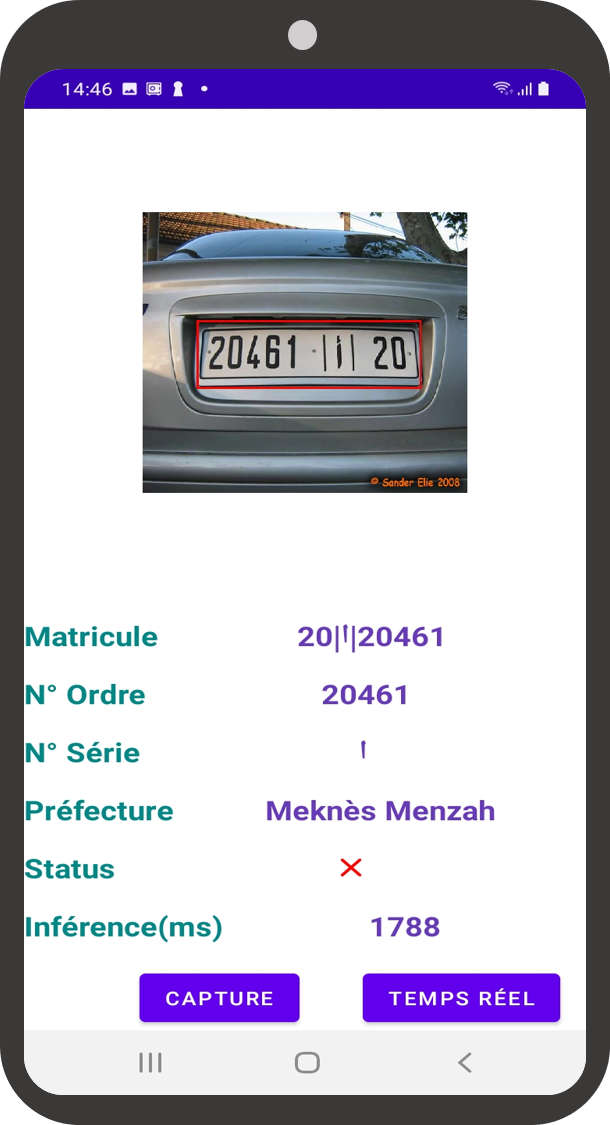
\includegraphics[width=\textwidth]{interface1.png}
        \caption{Exemple d'une reconnaissance de plaque non enregistrée dans la base de données réalisée en 1788 ms}
    \end{subfigure}
    \hfill
    \begin{subfigure}{0.3\textwidth}
        \centering
        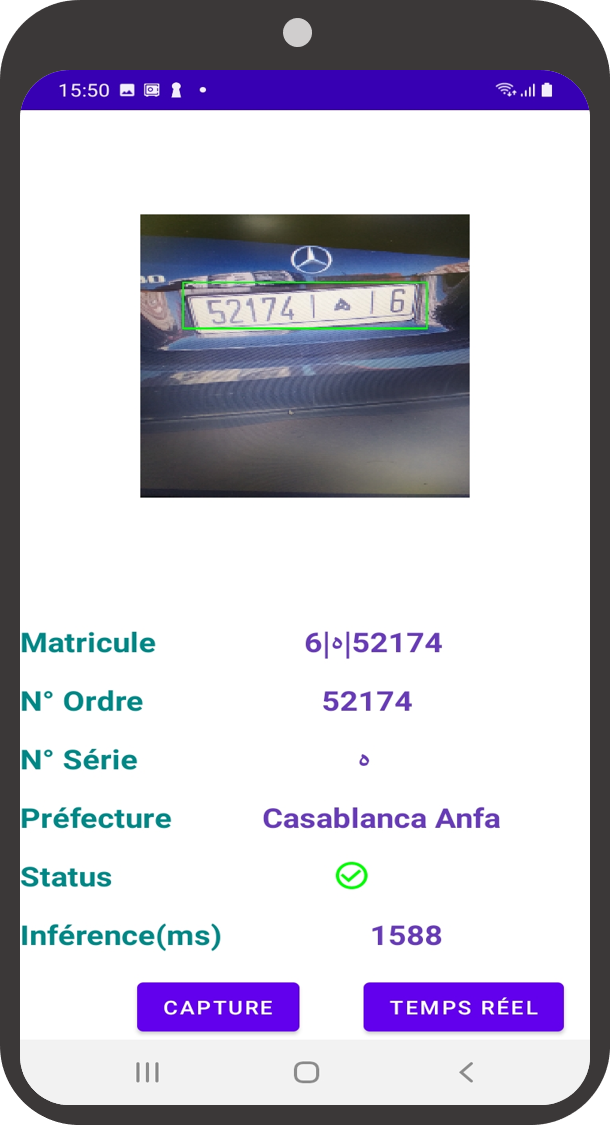
\includegraphics[width=\textwidth]{interface2.png}
        \caption{Exemple d'une reconnaissance de plaque enregistrée dans la base de données réalisée en 1588 ms}
    \end{subfigure}
    \caption{Exemples de quelques interfaces de l'application mobile}
\end{figure}



    \section{Parking intelligent}
Une des applications pratiques et très utiles du système ANPR est le parking intelligent ou encore smart parking. Entrant dans le cadre de la mobilité intelligente pour les citées dites intelligentes, les smart parking sont  une solution à la fois moderne et efficace pour résoudre le problème de stationnement dans les villes à forte agglomération et mobilité comme Casablanca ou Rabat. La solution développée par l’entreprise KF2Y Consulting se veut innovante car utilise les nouvelles techniques de Machine Learning à la place de capteurs ou carte RFID. Au cours de notre stage, une équipe de stagiaires étudiants en développement logiciel,système embarqué et services numériques et Machine Learning sous la coordination d’un responsable a mis en place une maquette plus ou moins réaliste d’un smart parking. 

    \subsection{Architecture du système GoPark}
Le système GoPark est constitué principalement de deux grandes parties communiquant entre elles via les services web à travers les requêtes HTTP: 
    \begin{itemize}
        \item L’\textbf{application mobile GoPark}: c’est une application qui permet d’une part à des clients propriétaires de Parking de créer des annonces de location de places sur son Parking. D’autre part, elle permet à d’autres clients véhiculés d’effectuer des réservations de stationnement sur l’un des parkings présents dans les annonces. Par ailleurs, c'est une application multi plateforme développée par les étudiants en ingénierie logiciel du groupe en utilisant le kit de développement logiciel Flutter.
        \item Le \textbf{système embarqué}: c’est un ensemble des composants électroniques et informatiques qui seront installés sur le parking pour la gestion automatique du stationnement. Dans le cadre de notre projet, notre système embarqué peut être subdivisé en deux grandes parties: la \textbf{barrière intelligente} qui donne accès ou non aux places de stationnement en fonction du numéro de matricule reconnu et le \textbf{détecteur de stationnement} qui permet signaler à l'application mobile la disponibilité d'une place du parking.
    \end{itemize}
    Dans les prochaines lignes, nous allons plus nous focaliser sur le système embarqué, la partie de l'application mobile ne faisant partie de nos domaines d'intervention durant notre période de stage. 
    \begin{figure}
        \centering
        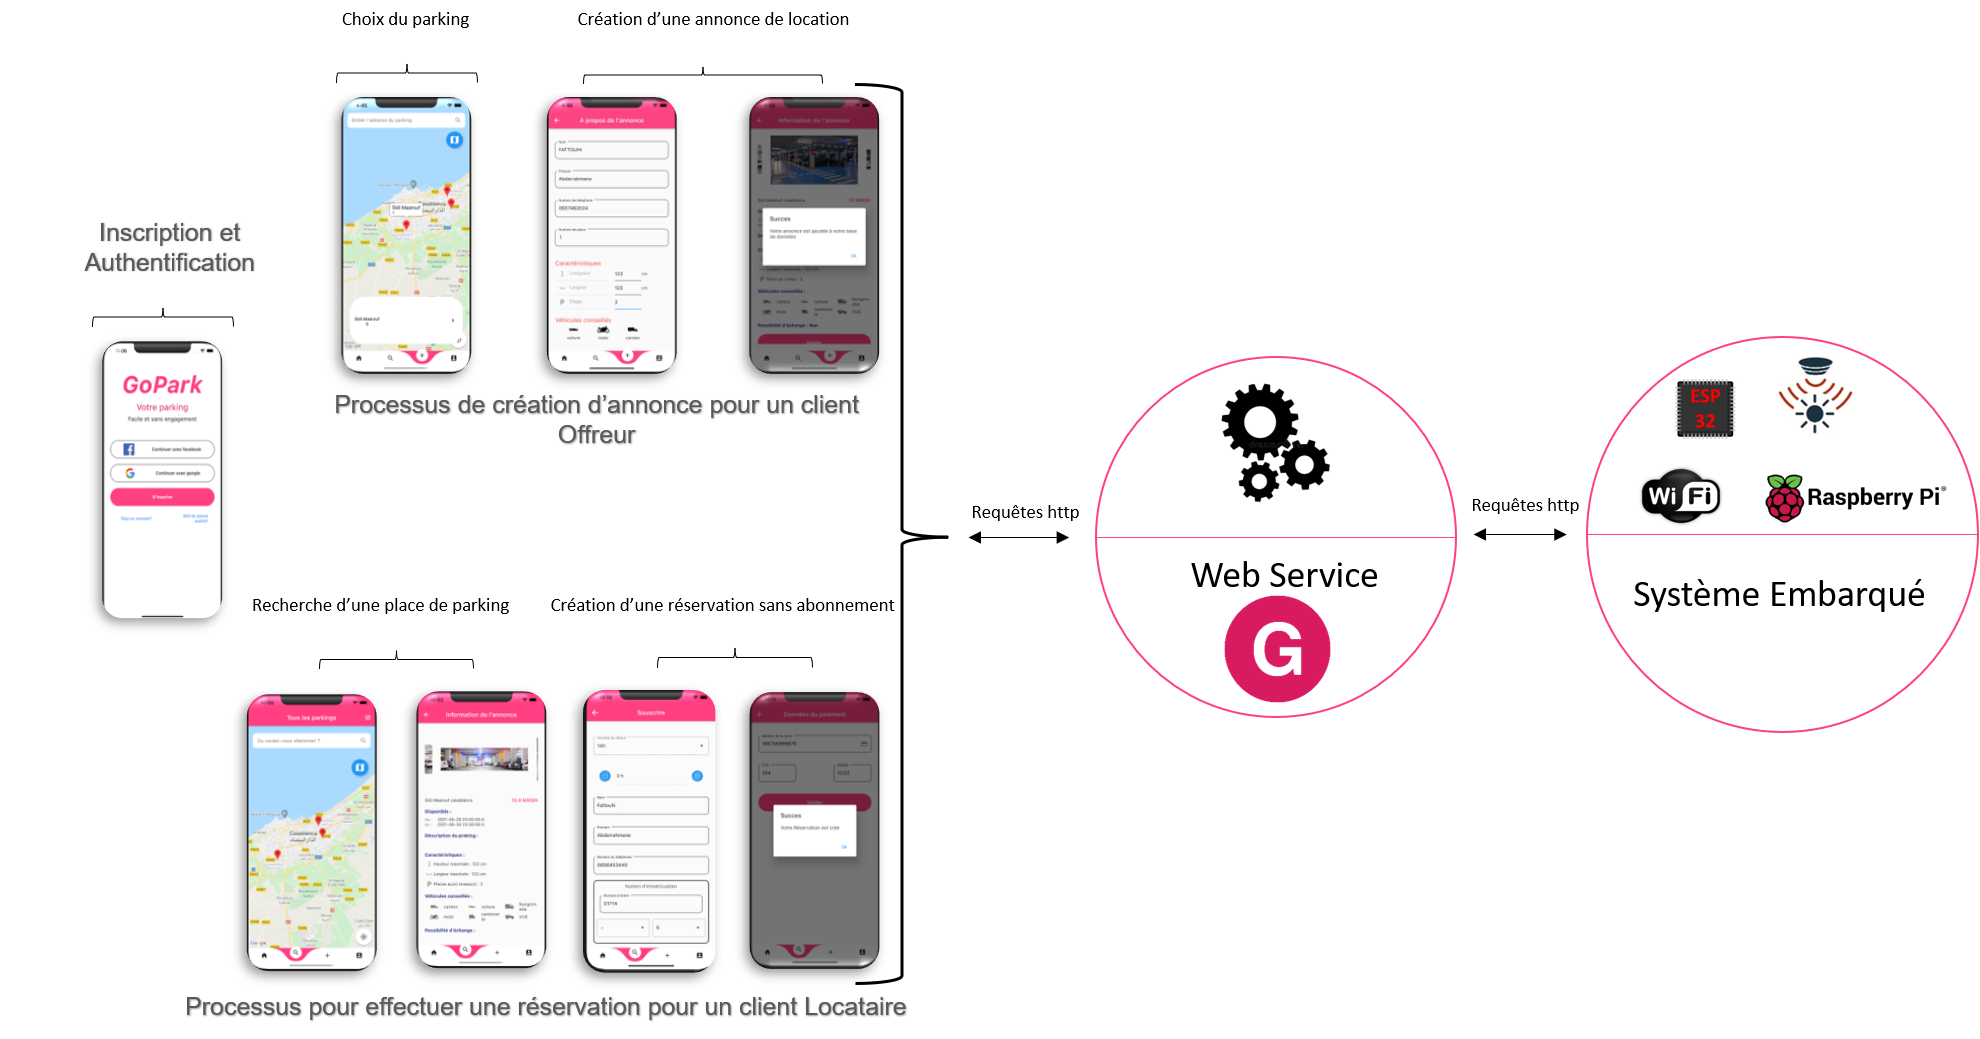
\includegraphics[scale=0.5]{goParkArchitecture.png}
        \caption{Architecture du système GoPark}
    \end{figure}

    \subsection{Environnements materiel et logiciel}
    La réalisation de la maquette de GoPark a été possible grâce à la combinaison d’un assez grand nombre d’outils matériels et logiciels. Parmi les outils matériels, on retrouve:
    \begin{enumerate}
        \item Des \textbf{capteurs ultrasoniques (1)}: ils permettent de détecter la présence d’un objet et dans notre cas la présence d’un véhicule dans l’espace de stationnement. Son principe comme son nom l’indique repose sur l’utilisation des ultrasons (ondes acoustiques). Ils sont composés d’un émetteur et d’un récepteur. L’émetteur émet régulièrement un train d’ondes qui va se réfléchir sur l’objet détecté et ensuite se rediriger vers le récepteur. Pour les deux places disponibles dans notre maquette, nous avons utilisé deux capteurs ultrasoniques.
        \item Des \textbf{microcontrôleurs (2)}: ce sont des circuits intégrés qui se composent des éléments essentiels et minimaux d’un ordinateur(processeur, mémoires, unité périphérique et interfaces entrées/sorties). Ils ont été utilisés pour le traitement avec les capteurs ultrasoniques et communiquer ainsi au serveur de l’application mobile les résultats de la détection de présence.
        \item Un \textbf{servomoteur SG90 (3)}:  c’est un actionneur qui déclenche un mouvement précis suite à une commande externe. C’est le composant qui servira à l’ouverture et la fermeture de la barrière de notre parking.
        \item Une \textbf{carte Raspberry Pi 4 (4)}: c'est un petit ordinateur (nano ordinateur) de la taille d'une carte de crédit offrant toutes les fonctionnalités d’un ordinateur standard. C’est dans cette carte que nous allons déployer notre système de reconnaissance des plaques d’immatriculation marocaines. A cette carte seront connectés le servomoteur SG90 et une \textbf{caméra V2 de 8 mégapixels (5)} pour récupérer les images de l’entrée du parking en temps réel. Voici quelques spécifications de la carte Raspberry Pi 4 que nous avons utilisée:
        \begin{table}[H]
            \centering
            \begin{tabular}{|l|l|}
                \hline
                \rowcolor{Gray}
                \textbf{Spécifications} & \textbf{Raspberry Pi 4} \\ \hline
                CPU & \textbf{1,5 GHz quadricœur ARM Cortex-A72} \\ \hline
                GPU & \textbf{Broadcom VideoCore VI, OpenGL ES 3.0} \\ \hline
                Puissance nominale  & \textbf{3A/15W} \\ \hline
                Systèmes d’exploitation & \textbf{Raspbian OS} \\ \hline
            \end{tabular}
            \caption{Spécifications de la carte Raspberry Pi 4}
        \end{table}
    \end{enumerate}
    \begin{figure}
        \centering
        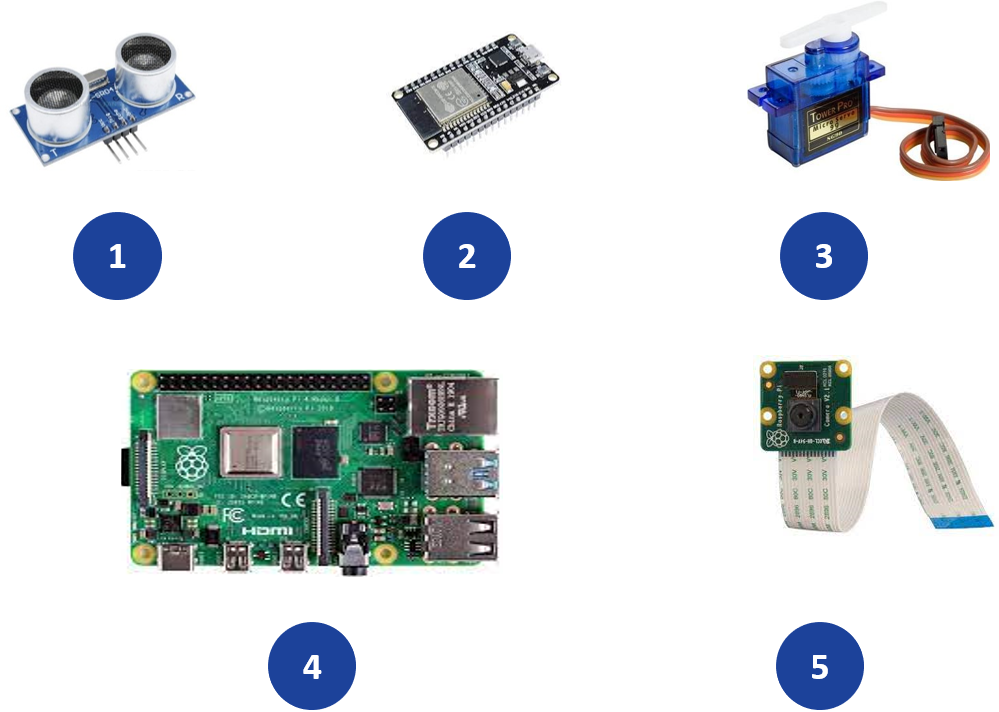
\includegraphics[scale=0.5]{materielGoPark}
        \caption{Outils matériels pour la réalisation du parking intelligent}
    \end{figure}

    Du côté logiciel, les outils dont nous nous sommes servis sont:
    \begin{enumerate}
        \item L’\textbf{IDE Arduino}: c’est une application multiplateforme qui permet d’écrire et de télécharger des programmes sur les cartes compatibles Arduino. Nous l’avons utilisé pour programmer les traitements opérés par le microcontrôleur. 
        \item Le \textbf{langage de programmation C++}: c’est le langage utilisé pour coder les programmes sous Arduino.
        \item \textbf{Firebase}: c’est un ensemble de services d’hébergement pour les divers types d'applications. Nous l’avons utilisé pour le service de base de données NoSQL qui stocke en temps réel l’état d'une place envoyée par le microcontrôleur.
        \item \textbf{Python}: c’est un langage de programmation interprété, multi-plateforme et multi paradigme. Au vu de sa simplicité et de la grande documentation disponible, nous avons opté pour ce langage pour coder nos programmes sur la carte Raspberry. 
        \item \textbf{OpenCV}: c’est une bibliothèque regroupant plusieurs fonctions de traitement d’images. Elle a été utile pour exécuter les différents modèles de détection et de lecture des plaques d'immatriculation sur les images en temps réel envoyées par la caméra.
        \item L’\textbf{IDE Thonny}: c'est l'éditeur utilisé pour le codage en Python.
    \end{enumerate}
    \begin{figure}
        \centering
        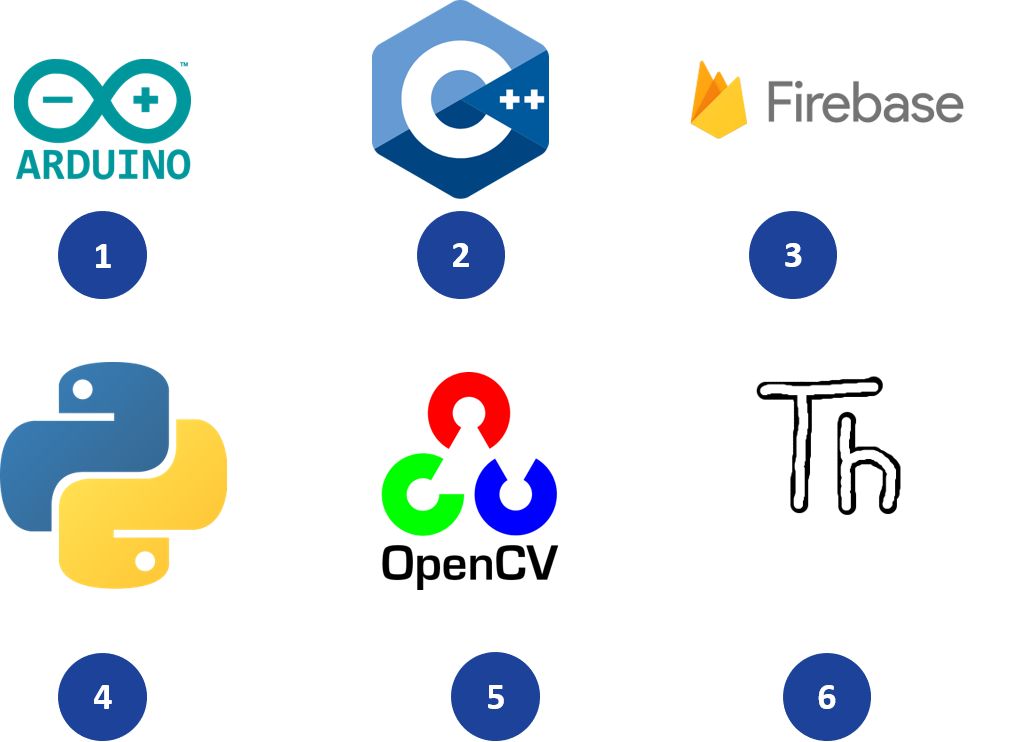
\includegraphics[scale=0.5]{logicielGoPark.png}
        \caption{Outils logiciels pour la réalisation du parking intelligent}
    \end{figure}

    \subsection{Résulats}
Le smart parking matérialisé par la maquette \ref{fig:maquette} et réalisé par notre équipe de stagiaire de KF2Y Consulting fonctionne en plusieurs étapes comme le montre la figure \ref{fig:fonctionnement}:
    \begin{enumerate}
        \item \textbf{Création d’une annonce de parking}: on accède à l’application mobile et on crée une annonce sur un parking en indiquant les places disponibles et le lieu;
        \item \textbf{Création d’une réservation}: on (en réalité un client véhiculé )accède à l’application et fait une réservation d’une place disponible pendant une tranche horaire dans un parking présent dans les annonces sans oublier de spécifier le numéro de matricule du véhicule;
        \item \textbf{Lecture de la plaque d'immatriculation}: le véhicule se dirige à l’entrée du parking où se trouve une caméra et une barrière intelligente. La caméra envoie au programme s'exécutant sur la carte Raspberry l’image du véhicule. Le programme localise dans un premier temps la position de la plaque et par la suite extrait sous format textuel le numéro du matricule;
        \item \textbf{Vérification de l'enregistrement du matricule}: le programme s'exécutant dans la carte envoie à travers les services web REST, le numéro de matricule détecté à l’application GoPark. L’application vérifie l’existence de ce matricule dans la base de données et renvoie la réponse au programme sur la carte;
        \item \textbf{Action sur la barrière}: Si la réponse reçue par la carte est positive, on ne déclenche aucune action sur la barrière donc elle reste fermée. Dans le cas contraire, le programme déclenche immédiatement l’ouverture de la barrière pour donner accès au véhicule à la zone de stationnement;
        \item \textbf{Signalisation de l’occupation d’une place}: lorsque le véhicule arrive sur sa place de stationnement, le capteur ultrason détecte sa présence et envoie une pulsion au microcontrôleur. Ce dernier signale  cette occupation à l’application GoPark via Firebase;
        \item \textbf{Signalisation de la libération d’une place}: au moment où le véhicule libère la place, les mêmes opérations précédentes sont faites par le capteur et le microcontrôleur mais cette fois-ci pour signaler la libération d'une place.
    \end{enumerate}
    \begin{figure}
        \centering
        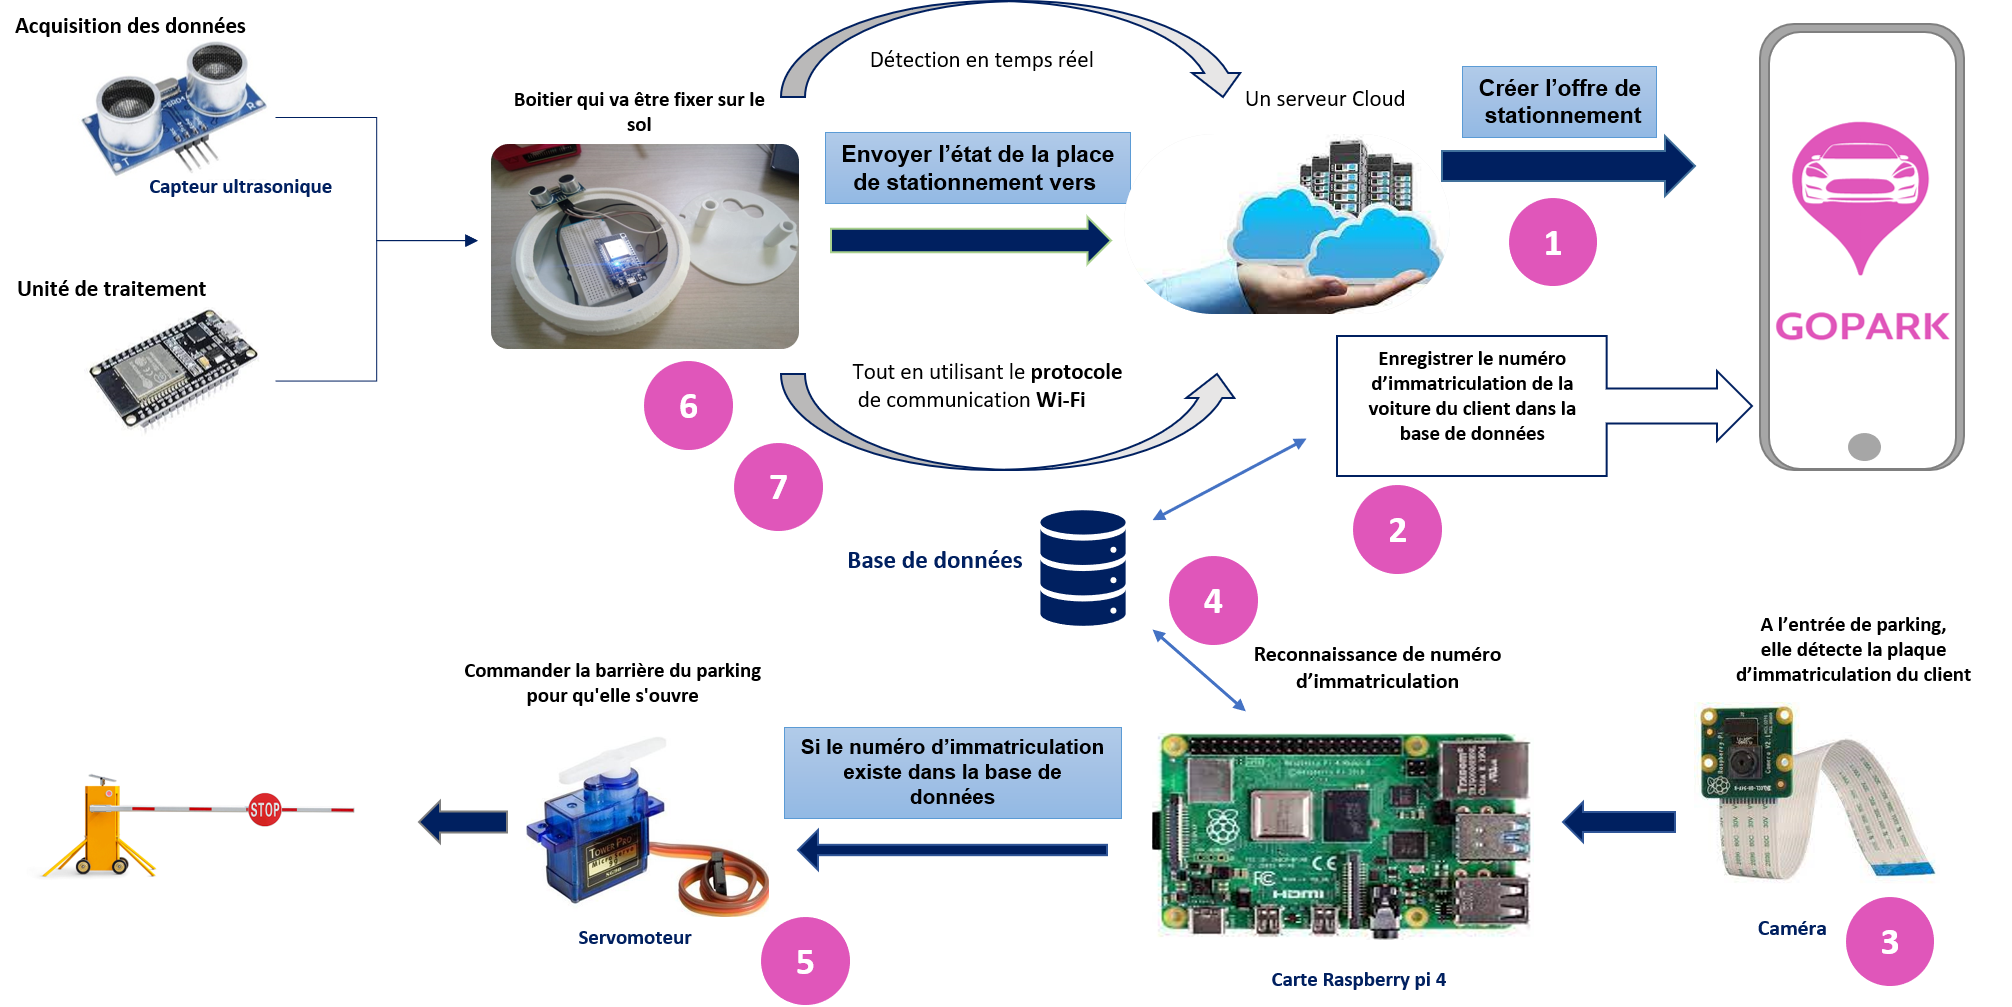
\includegraphics[scale=0.5]{goParkFonctionnement.png}
        \caption{Fonctionnement général de GoPark}
        \label{fig:fonctionnement}
    \end{figure}
    
    \begin{figure}
        \centering
        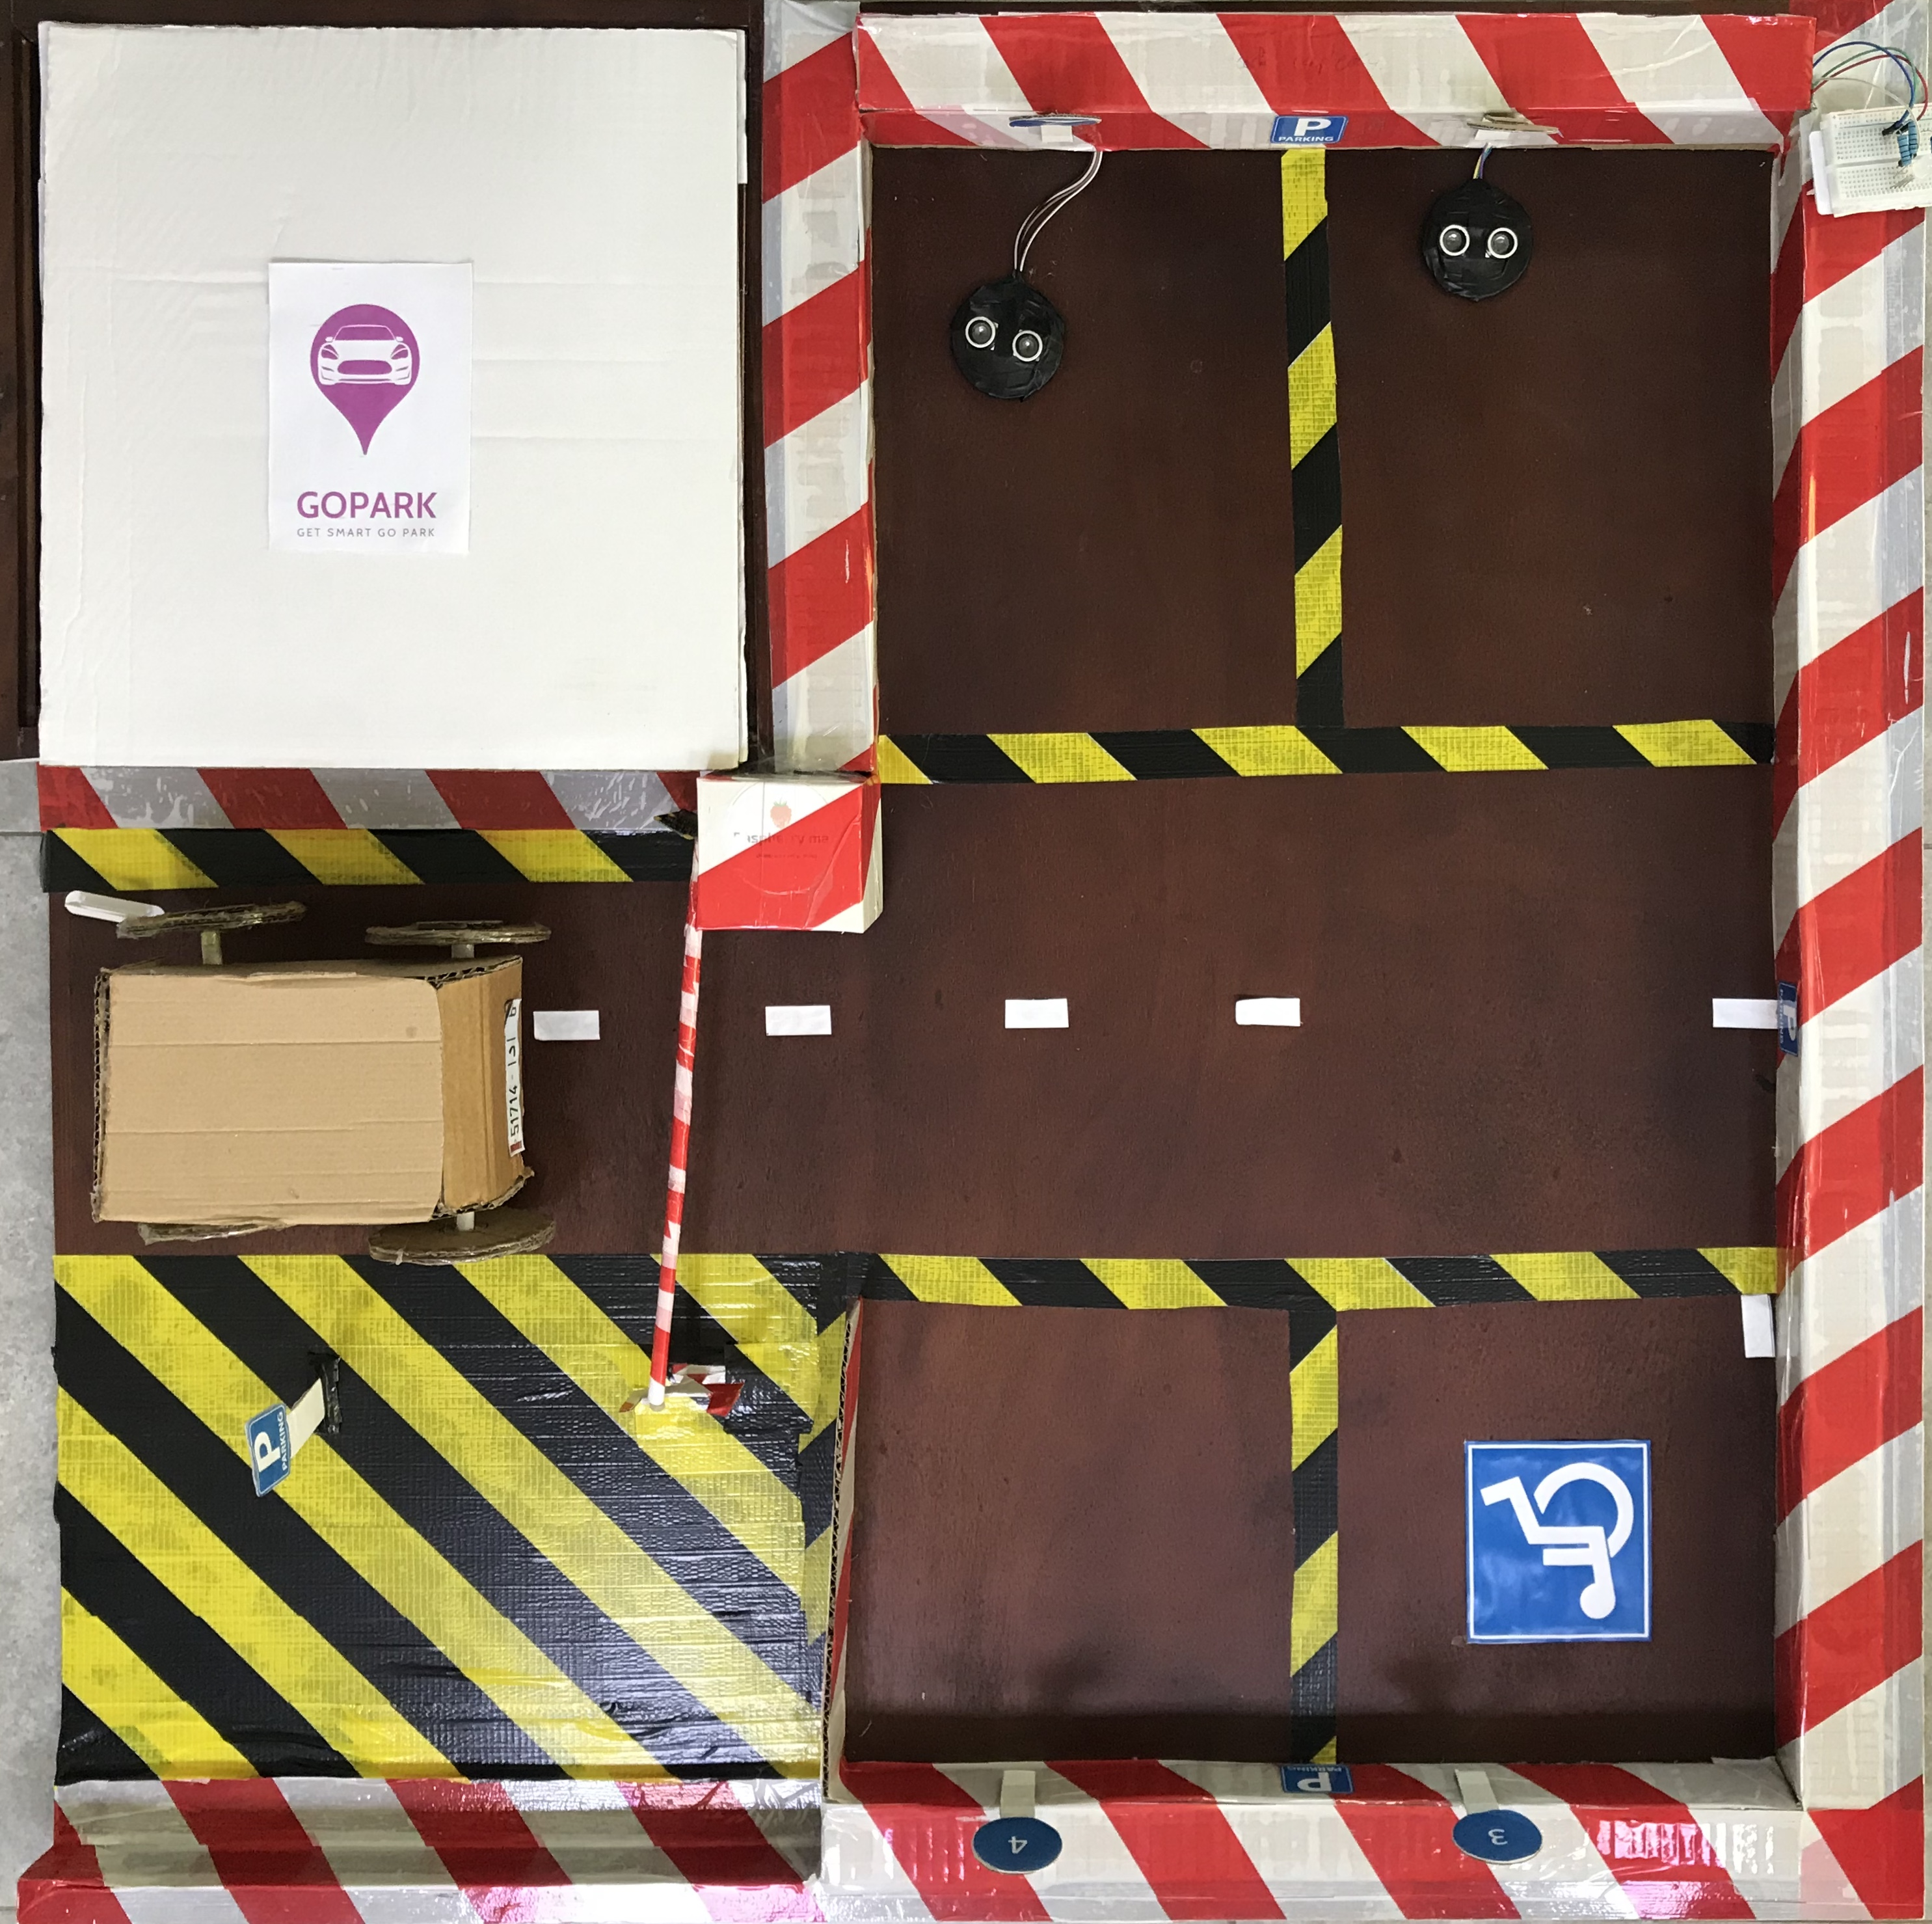
\includegraphics[width=500pt]{maquette}
        \caption{Maquette du parking intelligent GoPark}
        \label{fig:maquette}
    \end{figure}
    
    \section{Conclusion}
    Nous arrivons au terme de ce dernier chapitre qui nous a permis de présenter les différentes applications dans lesquelles nous avons déployé notre système ANPR SIRAM. La première est une application mobile qui permet de faire la reconnaissance des plaques d’immatriculation marocaines d’une part  sur une capture d’image prise par un utilisateur et d’autre part sur une vidéo en temps réel. La seconde est un parking intelligent appelé GoPark. Nous avons réalisé une maquette de ce parking qui utilise le système ANPR pour lire les plaques d’immatriculation des véhicules à l’entrée du parking. Le résultat donné par ce système permet de déterminer si on doit déclencher l’ouverture de la barrière ou non. Ce dernier chapitre loin d’être le moindre montre à quel point le système ANPR que nous avons développé peut être utile pour notre société et faciliter ainsi la circulation et le stationnement dans de grandes métropoles du Royaume comme Casablanca. 
